\chapter{新闻事件的主题演化分析方法研究}
第二章,我们介绍了文本分析的常用方法,以及它们在具体场景的应用。然而这些方法并没有考虑文本的产生的时间,在建模时简单认为文本之间是可交换的。显然这样的处理方式不够充分,因为在现实情况中,大部分文本(如,新闻报道,学术文章)都具有时间属性。对同一事物或事件的叙述,随着时间的推移一定会产生变化,而这些变化之间的差异又必然会存在一定的依赖的关系。本章,我们将重点研究新闻语料的特点,并基于此提出一套有效的方法来跟踪新闻事件的主题演化过程。

\section{新闻事件的时序分析}
\subsection{新闻报道的时序分布}
当某一重大新闻事件$E_1$爆发时,通常在较短的时间内,各大媒体都会争相报道,此时关于此事件的报道数量会迅速达到一个峰值$P_1$。随着时间的该事件开始慢慢降温,或者发生了其他更具吸引力的事件$E_2$发生了,那么关于事件$E_1$的报道数量也会回落到一个较小的范围。然而,对于重要的新闻事件,随着时间的发展,不时会有新的信息被披露,每一次信息的披露都会让该事件重新获得上头条的机会,那么新闻的报道数量也就会重新攀升至一个新的峰值$P_2$。如此往复,重大新闻事件往往会经历几个阶段。

如果我们将事件$E_1$每次报道数量达到峰值前后一段时间一起作为一个 \emph{阶段},虽然在这个阶段内新闻的报道数量会非常多,但是实际上大部分的报道内容都非常的相似,因为各家媒体获得信息都差不多。然后,不同的阶段之间,报道的内容会有较大的不同。我们从英国卫报\emph{The Guardian}上分别抓取了以 \emph{Edward Snowden}和\emph{Obamacare}为关键词的新闻报道,\textbf{Figure.\ref{temporal distribution}} 表示他们的时序分布。正如我们的猜想,新闻报道的实际时序分布的确包含了多个波峰和波谷。

% BEGIN == 新闻报道的时序分布图
\begin{figure}[htb]
	\subfigure[Edward Snowden]{
		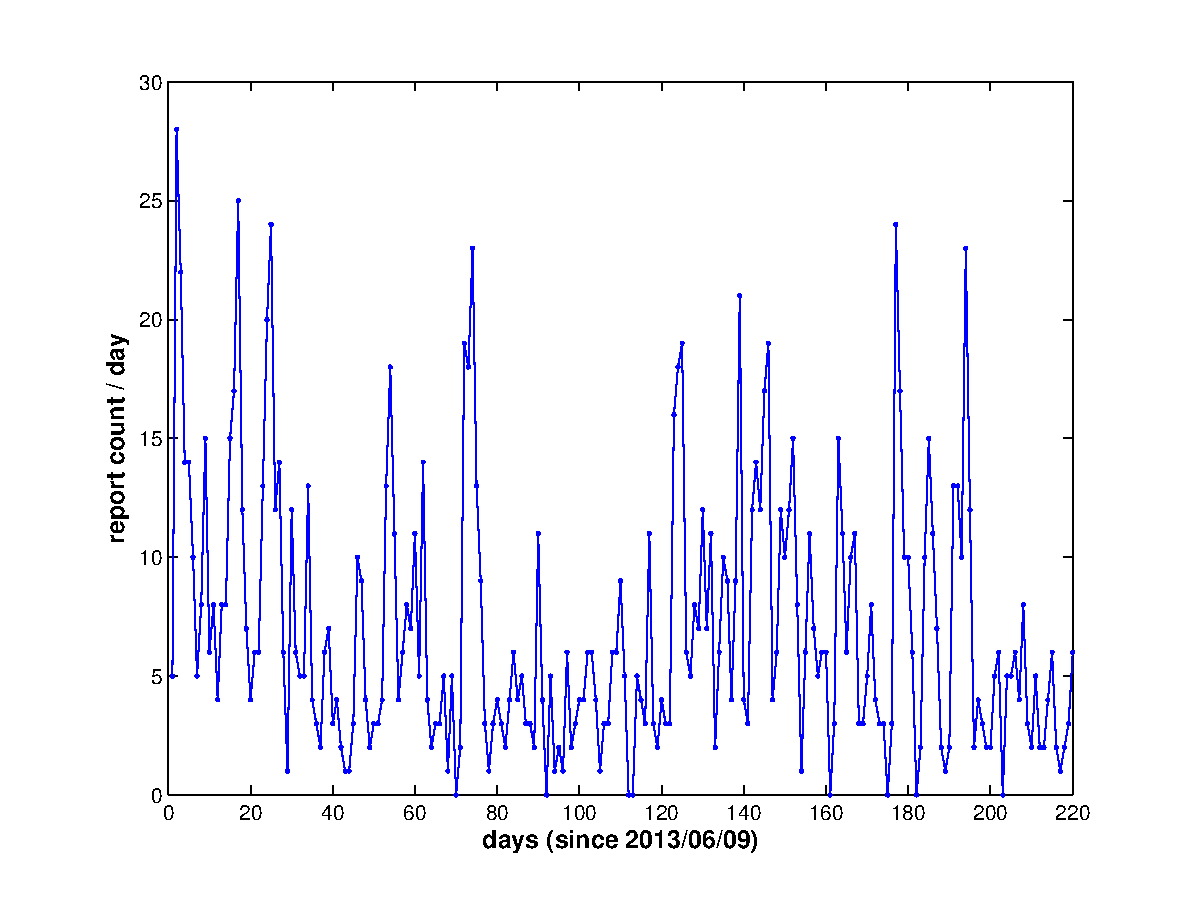
\includegraphics[width=7.5cm]{guardian_snowden}
		\label{temporal distribution:snowden}
	}
	\subfigure[Obamacare]{
		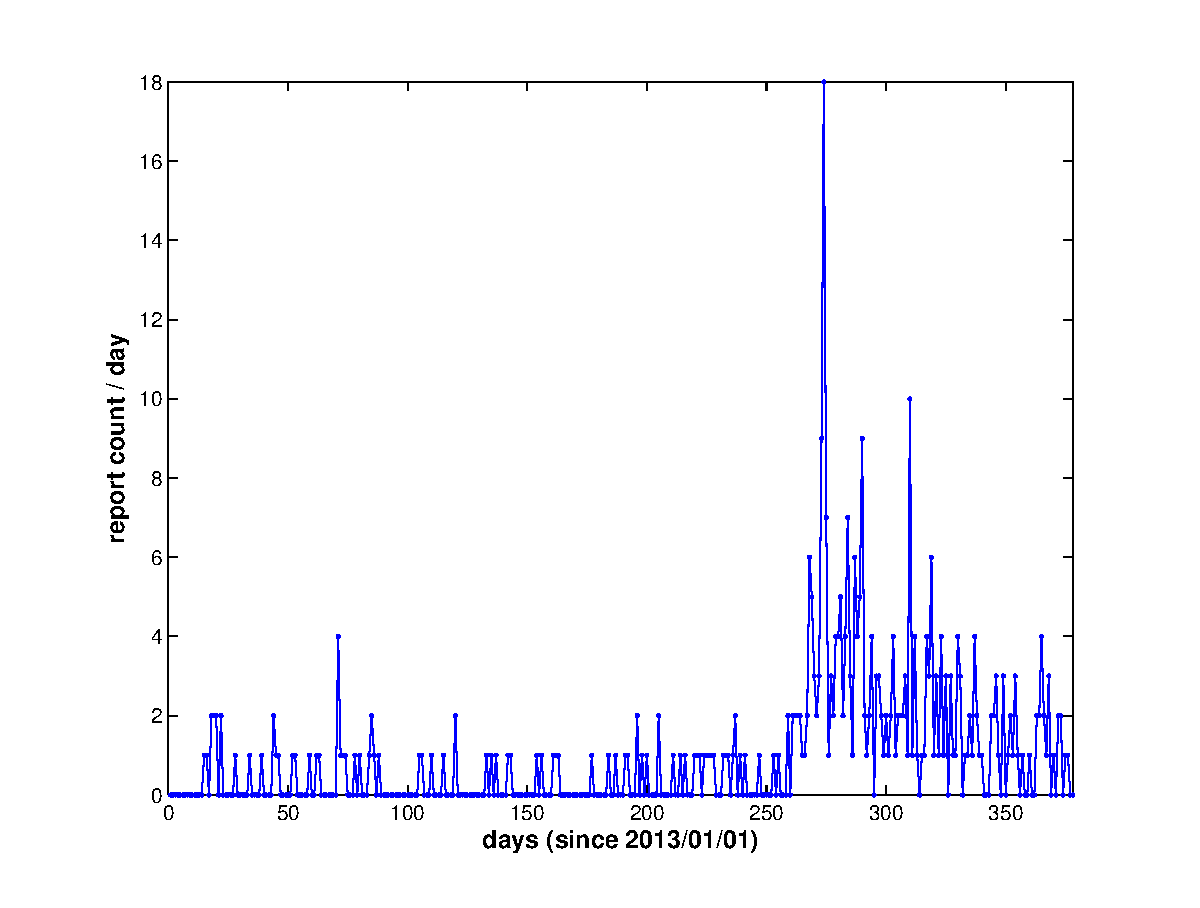
\includegraphics[width=7.5cm]{guardian_obamacare}
		\label{temporal distribution:obamacare}
	}
	\caption{关于"Edward Snowden" 和 "Obamacare" 相关新闻的报道数量时序分布图. X轴表示时间(单位:天),Y轴表示新闻的报道数量(单位:篇)}
	\label{temporal distribution}
\end{figure}
% END == 新闻报道的时序分布图

\subsection{新闻语料的时序划分}
DTM \cite{Blei:2006}是由David Blei等人提出的动态主题模型,该模型将语料库均匀(如按年,月,日等)划分为多个子集,由此获得的每个子集时间跨度都相同。然而,根据我们上一小节分析的可以知道,均匀划分语料库的方法显然有许多不妥之处。首先,各个子集的文本数量上可能会有很大的差异,有的子集文本数量非常多,有点非常少;其次,均匀划分时前后时间段的分割点,可能恰好落在 \textbf{Figure.\ref{temporal distribution}} 所示的波峰位置,这样就把一堆一致性非常高的文本划分到了两个阶段。

基于上面的分析,我们可以得到一个合理的划分语料库所需满足的几个条件:首先,每个时间段内的文本具有较高的一致性,它们可能都是报道事件的同一个方面或同一个进展;第二,尽量保障每个时间段的文档数量不要太少。从 \textbf{Figure.\ref{temporal distribution}} 来看的话,一个好的分割点应该是落在波谷附近。

为了实现语料库的自动划分,我们设计了一个自适应的聚类算法 \emph{Adaptive K-Means Algorithm}. 该算法是基于K-Means \cite{kanungo2002efficient} 改进而来,弥补了K-Means需要手动设置聚类数的不足。该算法是一个迭代算法,每一次迭代将聚类数目加1,并且计算本次迭代结束后,聚类中所有点离其中心点的\textbf{\emph{加权平均距离 Weighted Mean Distance}},该距离公式定义如下:
\begin{equation}\label{eq:wmd}
Weighted\;Mean\;Distance=\frac{\sum_{i=1}^{n}{mean\;distance\;of\;cluster\;i}}{n}
\end{equation}
每次迭代结束后,将当前的加权平均距离$WMD_i$与前一次迭代获得的加权平均距离$WMD_{i-1}$相减,若\emph{加权平均距离}的减少量达到预设的阀值,则迭代结束,此时的聚类数目便是最佳的聚类数。\textbf{公式 \ref{eq:wmd}} 中的距离使用的是二维空间中的\emph{欧式距离}, 算法的为代码描述如下:

% BEGIN == 自适应聚类算法 伪代码
\begin{algorithm}
  \DontPrintSemicolon
  \KwData{$X$: news count of each day; $max\_k$: the maximum value of K; $t$: threshold value}
  \KwResult{$count$: article count of each episode; $dists$: weighted mean distance array; $K$: the best count of cluster}
  \BlankLine
  $Y \longleftarrow$ remove $zero$ points from $X$\;
  \For{$i \leftarrow 1$ \KwTo $max\_k$}{
    $[count, sumd]=kmeans(Y, i)$;\;
    \tcp*[r]{$count$: point count of each cluster}
    \tcp*[r]{$sumd$: sum distance of each cluster}
    $means \leftarrow calc\_mean\_distance(count, sumd)$;\;
    \tcp*[r]{$means$: mean distances of all clusters}
    $dists[i] \leftarrow calc\_weighted\_mean\_distance(means)$;\; 
    \If{$i > 1$} {
      \If{$dists[i]-dists[i-1] < t$}{
        $K \leftarrow (i-1)$; break;
      }
    }
  }
  \If{$K = 0$} {$K \leftarrow max\_k$;\;}
  \caption{Adaptive K-Means algorithm}
  \label{algorithm1}
\end{algorithm}
% END == 自适应聚类算法 伪代码

\subsection{主题相似度计算}
As is defined above, the main topic is the one which has the most similarities between two adjacent episodes. In order to discover the main topic and track the evolution, we need to calculate the similarity between adjacent episodes. As the topic is characterized by a distribution over words. A simple measure method of similarity between topics is the \emph{Kullback-Leibler divergence} (also called \emph{relative entropy}). For discrete probability distribution $P$ and $Q$, the \emph{KL divergence} is defined to be
\begin{equation}
D_{KL} \left ( P||Q \right ) = \sum_{i}ln\left ( \frac{P(i)}{Q(i)} \right ) P(i)
\end{equation}
However, the \emph{KL divergence} is not a proper distance measure method because it is not symmetric. An alternative option is the \emph{Jensen-Shannon distance}, which is a smoothed and symmetric extension of the \emph{KL divergence}.
\begin{equation}
D_{JS} \left ( P||Q \right ) = \frac{1}{2} D_{KL} \left ( P||M \right ) + \frac{1}{2} D_{KL} \left ( Q||M \right )
\end{equation}
With the averaged variable $M = \frac{1}{2}(P+Q)$. 

\subsection{文本一致性及其度量}
\textbf{\emph{文本一致性 Coherence}} 度量的是文本之间主题的相似性。两个文本的一致性越高,表示这两篇文本的描述的内容越相似。从直觉角度出发,通常如果有一堆文本,如果这堆文本相互之间的一致性越高,那么用主题模型对文档集合进行建模时,能够挖掘的信息也就越丰富。以 \textbf{Figure.\ref{temporal distribution}} 中我们抓取的两个事件的新闻报道为例,方法一:我们将所有的报道全部作为一个集合进行主题挖掘;方法二,我们将各自事件的报道分开作为两个集合,分别进行主题挖掘。那么很显然方法二,所能挖掘出来的信息会更具体,我们能从方法二获得的事件的信息更多。

换言之,如果我们在使用主题模型进行文本分析时,如果在同一个时间区间内的文本之间一致性越高,那么结果就会更显著,对事件的理解也会更深入。通常我们可以利用\emph{方差}来度量数据的一致性,但是它却不能很好的体现文本主题的一致性,因此我们通过\textbf{\emph{主题覆盖率 n Topic Coverage Rate ($TCR_n$)}}来间接的度量,定义如下:
\begin{equation}
TCR_n = \frac{\left \| articles\;\;belong\;to\;these\;n\;topics \right \|}{\left \| all\;articles \right \|} * 100\%
\end{equation}
\label{eq:tcr}
在\textbf{公式 \ref{eq:tcr}} 中,$\left \| \cdot \right \|$表示集合中元素的数量,$TCR_n$度量最相关的前n个主题对文本的覆盖率。从公式 \textbf{公式 \ref{eq:tcr}} ,我们可知,如果主题数$n$固定,那么$TCR_n$越大,文本之间的的一致性越高;同时,若$TCR_n$固定,那么主题数$n$越小,文本之间的一致性越高。
























